\documentclass[12pt,twoside]{article}
\usepackage{graphicx}
\usepackage[british]{babel}
\usepackage{amssymb}
%
% use the next three lines to control the position of the
% text inside the paper sheet.
%
 \voffset=-12mm       % vertical displacement
 \oddsidemargin=3mm   % horizontal displacement (odd pages)
 \evensidemargin=3mm  % horizontal displacement (even pages)
%
 \textwidth=160mm
 \textheight=225mm
%
% capcelera
%
\title{A software package for the numerical integration of ODEs by
       means of high-order Taylor methods}
%
\author{\`Angel Jorba$^{(1)}$ and Maorong Zou$^{(2)}$}
%
\pagestyle{myheadings}
%
% entorns
%
\newtheorem{definition}{Definition}[section]
\newtheorem{lemma}{Lemma}[section]
\newtheorem{proposition}{Proposition}[section]
\newtheorem{theorem}{Theorem}[section]
\newtheorem{corollary}{Corollary}[section]
\newtheorem{remark}{Remark}[section]
\newcommand{\bproof}{\noindent {\bf Proof:} }
\newcommand{\eproof}{\hfill $\rule{3mm}{3mm}$}
%
% simbols
%
\newcommand{\NN}{{\mathbb N}}               % for natural numbers
\newcommand{\ZZ}{{\mathbb Z}}               % for entire numbers
\newcommand{\QQ}{{\mathbb Q}}               % for rational numbers
\newcommand{\RR}{{\mathbb R}}               % for real numbers
\newcommand{\CC}{{\mathbb C}}               % for complex numbers
\newcommand{\TT}{{\mathbb T}}               % for the standard torus
\newcommand{\ii}{{\mbox{\rm i}\,}}            % imaginary unit
\renewcommand{\Re}{\mbox{\rm Re}\,}           % real part
\renewcommand{\Im}{\mbox{\rm Im}\,}           % imaginary part
\newcommand{\diag}{\mbox{\rm diag}}
\newcommand{\mod}{\mbox{\rm mod}\,}
\newcommand{\interior}[1]{\mbox{\raisebox{0.2ex}{$\stackrel{\circ}{#1}$}}}
\newcommand{\eps}{\mbox{\rm eps}}

\begin{document}
\selectlanguage{british}
\maketitle
\begin{itemize}
\item[(1)]
Departament de Matem\`atica Aplicada i An\`alisi,
Universitat de Barcelona,\newline
Gran Via 585, 08007 Barcelona, Spain.
E-mail: \texttt{angel@maia.ub.es}

\item[(2)]
Department of Mathematics,
The University of Texas at Austin,\newline
Austin, TX 78712-1082, USA.
E-mail: \texttt{mzou@math.utexas.edu}
\end{itemize}

\bigskip

\hfill\textit{To the memory of William F. Schelter}

\bigskip

\thispagestyle{empty}

\begin{abstract}
  This paper revisits the Taylor method for the numerical integration
  of initial value problems of Ordinary Differential Equations (ODEs).
  The main goal is to show that the Taylor method can be competitive,
  both in speed and accuracy, with the standard methods. To this end,
  we present a computer program that outputs an specific numerical
  integrator for a given set of ODEs. The generated code includes
  adaptive selection of order and step size at run time. The package
  provides support for several extended precision arithmetics,
  including user-defined types.
  
  The paper discusses the performance of the resulting integrator in
  some examples, showing that it is a very competitive method in many
  situations. This is specially true for integrations that require
  extended precision arithmetic. The main drawback is that the Taylor
  method is an explicit method, so it has all the limitations of these
  kind of schemes. For instance, it is not suitable for stiff systems.
\end{abstract}

\newpage

\tableofcontents

\newpage

%%%%
\markboth{Numerical integration of ODEs by means of Taylor methods}
{\`A. Jorba, M. Zou}
%%%%

\section{Introduction}
Let us consider the following problem: find a smooth function
$x:[a,b]\rightarrow\RR^m$ such that
\begin{equation}
\left\{
\begin{array}{lcl}
x'(t) & = & f(t,x(t)), \\
x(a) & = &x_0,
\end{array}
\right.
\label{eq:ivp}
\end{equation}
where $f:[a,b]\times\Omega\subset\RR\times\RR^m\rightarrow\RR^m$ is a
smooth function, $\Omega=\interior{\Omega}$ and $m\ge 1$. There is a
classical result of the theory of ODE that ensures the existence and
uniqueness of a function $x(t)$, defined on $[a,b_0]\subset[a,b]$,
satisfying (\ref{eq:ivp}). However, the effective computation of such
a function is a much more difficult question.

The search of good numerical methods for (\ref{eq:ivp}) is one of the
classical problems in numerical analysis. The usual procedures are
based on approximating the values $x(t)$ on a suitable mesh of values
of $t$. For the moment, and to simplify the presentation, we will use
an equispaced mesh and we will assume that $x(t)$ is defined on the
whole interval $[a,b]$. Therefore, if $M\in\NN$, we define
\[
h=\frac{b-a}{M},\quad t_m=a+mh,\quad 0\le m\le M.
\]
The problem now is to find approximations $x_m$ to the exact values
$x(t_m)$. The computation of these approximations $x_m$ is usually
performed recurrently from the (previously computed) values
$x_0,\ldots,x_{m-1}$. Each step of this recurrence is known as a time
step, and its computer implementation is also called a time-stepper.

In this paper we will revisit one of the oldest numerical procedures
for the numerical integration of ODEs: the Taylor method. For
simplicity, we will assume that the function $f$ is analytic for
$(t,x)\in[a,b]\times\Omega$. The idea of the method is very simple:
given the initial condition $x(t_m)=x_m$, the value $x(t_{m+1})$ is
approximated from the Taylor series of $x(t)$ at $t=t_m$. The
algorithm is then,
\begin{equation}
\begin{array}{rcl}
x_0 &=&x(a), \\
x_{m+1} &=& x_m+x'(t_m)h+\displaystyle\frac{x''(t_m)}{2!}h^2+\cdots+
   \displaystyle\frac{x^{(p)}(t_m)}{p!}h^p,
      \quad m=0,\ldots, M-1. \\
\end{array}
\label{eq:taylor-method}
\end{equation}
We refer to \cite{HairerNW00} for a discussion of the basic properties
of the method. One of the key points for a practical implementation is
the effective computation of the values of the derivatives
$x^{(j)}(t_m)$. A first procedure to obtain them is to differentiate
the first equation in (\ref{eq:ivp}) w.r.t. $t$, at the point
$t=t_m$. Hence,
\[
x'(t_m)=f(t_m,x(t_m)),\quad
x''(t_m)=f_t(t_m,x(t_m))+f_x(t_m,x(t_m))x'(t_m),
\]
and so on. Therefore, the first step to apply this method is, for a
given $f$, to compute these derivatives up to a suitable order. Then,
for each step of the integration (see (\ref{eq:taylor-method})), we
have to evaluate these expressions to obtain the coefficients of the
power series of $x(t)$ at $t=t_m$. Usually, these expressions will be
very cumbersome, so it will take a significant amount of time to
evaluate them numerically. This, jointly with the initial effort to
compute the derivatives of $f$, is the main drawback of this approach
for the Taylor method.

This difficulty can be overcomed by using the so-called {\em automatic
differentiation} (\cite{Beda59}, \cite{Weng64}, \cite{Moore66},
\cite{Rall81}, \cite{GriewankC91}, \cite{BischofCCG92},
\cite{BerzBCG96}, \cite{Griewank00}).  This is a procedure that allows
for a fast computation of the derivatives of a given function, up to
arbitrarily high orders. As far as we know, these ideas were first
used in Celestial Mechanics problems (\cite{Steffensen56},
\cite{Steffensen57}; see also \cite{Broucke71}).

An inconvenience of this method is that the function $f$ has to belong
to a special class; fortunately, this class is large enough to contain
the functions that appear in many applications. We also note that the
program that computes these derivatives by automatic differentiation
has to be specifically coded for each function $f$. This coding can be
either done by a human (see, for instance, \cite{Broucke71} for an
example with the $N$-body problem) or by another program (see
\cite{Beda59,Gibbons60a,ChangC94} for general-purpose computer
programs). An alternative procedure to apply the Taylor method can be
found in \cite{SavageauV87} and \cite{IrvineS90}.

One of the goals of this work is to present a software that, given a
function $f$ (belonging to a suitable class), generates a complete
time-stepper based on Taylor method. The generated code is ANSI C, but
we also provide a Fortran 77 wrapper for the main call to the
time-stepper.

A software package that performs a similar task is ATOMFT (written by
Y.F. Chang) that can be freely downloaded from the Internet (to get a
copy you can visit, for instance,
\verb-http://www.eng.mu.edu/corlissg/FtpStuff/Atom3_11/- and
retrieve the file \verb-atom3_11.tar.Z-). ATOMFT is written in
Fortran~77 and it reads Fortran-like statements of the system of ODEs
and writes a Fortran 77 program that is run to numerically solve the
system using Taylor series.

One of the nicest characteristics of Taylor method is the possibility
of using interval arithmetic to derive bounds for the total error of
the numerical integration. These ideas have been used in ATOMFT to
compute a step size that guarantees a prescribed accuracy, but using
the standard floating point of the computer instead of interval
arithmetic. We also want to note that the step size selections in
``usual'' numerical integrators (Runge-Kutta, Adams-Bashford, etc.)
are based on the asymptotic behaviour of the error, and they do not
provide true bounds for the truncation error of the method. On the
other hand, the derivation of the time step in ATOMFT is a substantial
part of the computing time, while an estimation based on the
asymptotic behaviour of the error is usually much faster.

Here, we have implemented a step size control based on an asympotic
estimate of the error. The main reason for this selection is that we
want to compete against the ``usual'' numerical integrators -- which
use similar step size control techniques. Moreover, as we will see
later, our software allows the user to plug in its own step size
control, so it is not difficult to implement different strategies.

For an efficient numerical integration, we need some knowledge of the
order $p\in\NN$ up to which the derivatives have to be computed, and
an estimate of the step size $h$, in order to have a truncation error
of the order of a given threshold value $\varepsilon$. We note that,
as we have to select the value of two parameters ($p$ and $h$), we can
ask for a second condition besides the size of the truncation error.
Here we have chosen to minimize the number of operations needed to
advance the independent variable $t$ in one unit (\cite{Simo01a}). We
have also coded the algorithms to do these tasks so that the output of
the program is, in fact, a complete numerical integrator --with
automatic order and step size control-- for the initial value problem
(\ref{eq:ivp}).

We have tested this Taylor integrator against some well-known
integration methods. The results show that Taylor method is a very
competitive method to integrate with the standard double precision
arithmetic of the computer. However, the main motivation for writing
this software is to address the need of highly accurate computations
in some problems of Dynamical Systems and Mechanics (see, for
instance, \cite{MartinezS99}, \cite{SimoV01a} and
\cite{Simo01}). Methods whose order is not very high (less than, say,
12) can be extremely slow for computations requiring extended
precision arithmetic. This is one of the strong points of the software
presented here: note that Taylor method does not need to reduce the
step size to increase accuracy; it can simply increase the order (see
Section~\ref{sec:hac}). As we will see, this allows to greatly reduce
the total number of arithmetic operations during the numerical
integration.

As any explicit scheme, the Taylor method is not suitable for stiff
equations because, in this case, the errors can grow too fast.
However, there are modifications of the Taylor method to deal with
these situations (\cite{Bart80a}, \cite{JalbertZ85},
\cite{KirlingerC92} and \cite{CorlissGHKPS97}). These modifications
have not been considered in our software.

In the paper we present the main details of our implementation. We
have tried to produce an efficient package, in the sense that the
produced Taylor integrator be as fast as possible. Moreover, we have
also included support for multiple precision arithmetic. We have done
several test to compare the efficiency and accuracy of the generated
Taylor routine against other numerical integrators.

There are several papers that focus on computer implementations of the
Taylor method in different contexts; see, for instance,
\cite{BartWZ70a}, \cite{CorlissC82}, \cite{ChangC94}
and~\cite{Hoefkens01}.  A good survey is \cite{NedialkovJC99} (see
also \cite{Corliss95}).

The package has been released under the GNU Public License, so
anybody with Internet access is free to get it and to redistribute
it. To obtain a copy, yo can visit the URLs

\begin{tabular}{ll}
\verb-http://www.ma.utexas.edu/~mzou/taylor/-  & (US)\\
\verb-http://www.maia.ub.es/~angel/taylor/-  & (Europe)
\end{tabular}

We note that the actual version of the package is written to run under
the GNU/Linux operating system. We do not expect major problems to run
it under any version of Unix, but we do not plan to write ports for
other operating systems.

The paper has been split as follows: Section~\ref{sec:auto} contains a
survey about automatic differentiation, Section~\ref{sec:dssc} is
devoted to the selection of step size and truncation degree,
Section~\ref{sec:si} gives some details about the software and
Section~\ref{sec:tests} provides some tests and comparisons.


\section{A short summary on automatic differentiation}\label{sec:auto}
Before starting with the discussion of the package, we will summarise
the main rules of automatic differentiation.

Automatic differentiation is a recursive procedure to compute the
value of the derivatives of certain functions at a given point (see
\cite{Moore66,Rall81}). The considered functions are those that can be
obtained by sum, product, quotient, and composition of elementary
functions (elementary functions include polynomials, trigonometric
functions, real powers, exponentials and logarithms).

\subsection{Rules of automatic differentiation}\label{sec:rules}
To simplify the discussion let us introduce the following notation: if
$a:t\in I\subset\RR\mapsto\RR$ denotes a smooth function, we call its
normalized $n$-th derivative to the value
\begin{equation}
a^{[n]}(t)=\frac{1}{n!}a^{(n)}(t).
\label{eq:def[]}
\end{equation}
where $a^{(n)}(t)$ denotes the $n$-th derivative of $a$ w.r.t. $t$.
In what follows, we will focus on the computation of the values
$a^{[n]}(t)$.

Assume now that $a(t)=F(b(t),c(t))$ and that we know the values
$b^{[j]}(t)$ and $c^{[j]}(t)$, $j=0,\ldots,n$, for a given $t$. The
next proposition gives the $n$-th derivative of $a$ at $t$ for some
functions $F$.

\begin{proposition}\label{prop:leibniz}
If the functions $b$ and $c$ are of class $C^n$, and
$\alpha\in\RR\setminus\{0\}$, we have
\begin{itemize}
\renewcommand{\itemsep}{0pt}
\item[{\rm 1.}] If $a(t)=b(t)\pm c(t)$, then
   $a^{[n]}(t)=b^{[n]}(t)\pm c^{[n]}(t)$.

\item[{\rm 2.}] If $a(t)=b(t)c(t)$, then
   $a^{[n]}(t)=\displaystyle\sum_{j=0}^n b^{[n-j]}(t)c^{[j]}(t)$.

\item[{\rm 3.}] If $a(t)=\displaystyle\frac{b(t)}{c(t)}$, then
   $a^{[n]}(t)=\displaystyle\frac{1}{c^{[0]}(t)}
   \left[ b^{[n]}(t)-\sum_{j=1}^n c^{[j]}(t) a^{[n-j]}(t)\right]$.

\item[{\rm 4.}] If $a(t)=\displaystyle b(t)^{\alpha}$, then
   $a^{[n]}(t)=\displaystyle\frac{1}{nb^{[0]}(t)}
   \sum_{j=0}^{n-1}\left(n\alpha-j(\alpha+1)\right)b^{[n-j]}(t)a^{[j]}(t)$.

\item[{\rm 5.}] If $a(t)=\displaystyle e^{b(t)}$, then
   $a^{[n]}(t)=\displaystyle\frac{1}{n}
   \sum_{j=0}^{n-1}\left(n-j\right)a^{[j]}(t)b^{[n-j]}(t)$.

\item[{\rm 6.}] If $a(t)=\ln b(t)$, then
   $a^{[n]}(t)=\displaystyle\frac{1}{b^{[0]}(t)}\left[
   b^{[n]}(t)-\frac{1}{n}\sum_{j=1}^{n-1}(n-j)b^{[j]}(t)a^{[n-j]}(t)
   \right]$.

\item[{\rm 7.}] If $a(t)=\cos c(t)$ and $b(t)=\sin c(t)$, then
   \[
   a^{[n]}(t)=-\frac{1}{n}\sum_{j=1}^{n}jb^{[n-j]}(t)c^{[j]}(t),\quad
   b^{[n]}(t)= \frac{1}{n}\sum_{j=1}^{n}ja^{[n-j]}(t)c^{[j]}(t).
   \]
\end{itemize}
\end{proposition}

\bproof These proofs can be found in the literature, so we only give
some hints about them.
\begin{itemize}
\renewcommand{\itemsep}{0pt}
\item[{\rm 1.}] Obvious.

\item[{\rm 2.}] It follows from Leibniz's formula:
   \[
   a^{[n]}(t)= \frac{1}{n!}a^{(n)}(t)=
   \frac{1}{n!}\sum_{j=0}^n {n\choose j} b^{(n-j)}(t)c^{(j)}(t)
    = \sum_{j=0}^n b^{[n-j]}(t)c^{[j]}(t).
   \]

\item[{\rm 3.}] Apply item~2 to $a(t)c(t)=b(t)$.

\item[{\rm 4.}] Take logarithms and derivatives to obtain
$a'(t)b(t)=\alpha a(t)b'(t)$. Use item~2 and (\ref{eq:def[]}).

\item[{\rm 5.}] Take logarithms and derivatives to obtain
$a'(t)=a(t)b'(t)$. Use item~2 and (\ref{eq:def[]}).

\item[{\rm 6.}] Take derivatives to obtain $a'(t)b(t)=b'(t)$. Use
item~2 and (\ref{eq:def[]}).

\item[{\rm 7.}] Take derivatives to obtain $a'(t)=-b(t)c'(t)$ and
$b'(t)=a(t)c'(t)$. Use item~2 and~(\ref{eq:def[]}).
\end{itemize}
\eproof

\begin{remark}
It is possible to derive similar formulas for other functions, like
inverse trigonometric functions.
\end{remark}

\begin{corollary}\label{coro:nu-op}
The number of arithmetic operations to evaluate the normalized
derivatives of a function up to order $n$ is $O(n^2)$.
\end{corollary}

\bproof The number of operations to obtain the $j$-th derivative once
we know the previous ones is $O(j)$. Hence, the total number of
operations is $\sum_{j=1}^n O(j)=O(n^2)$.
\eproof

\medskip

Although these methods only allow for the derivation of a reduced
subset of the set of analytic functions, we note that they cover the
situations found in many applications.

\subsection{An example: The Van der Pol equation}
These rules can be applied recursively so that we can obtain recursive
formulas for the derivatives of a function described by combination of
these basic functions. As an example, we can apply them to the Van der
Pol equation,
\[
\left.
\begin{array}{rcl}
x'&=&y\\
y'&=&(1-x^2)y-x
\end{array}
\right\}.
\]
To this end we decompose the right-hand side of these equations in a
sequence of simple operations:
\begin{eqnarray}
\left.
\begin{array}{rcl}
u_1 & = & x\\
u_2 & = & y\\
u_3 & = & u_1 u_1\\
u_4 & = & 1-u_3\\
u_5 & = & u_4 u_2\\
u_6 & = & u_5-u_1\\
x'  & = & u_2\\
y'  & = & u_6
\end{array}
\right\}
\label{eq:vanderpol-decom}
\end{eqnarray}
Then, we can apply the formulas given in
Proposition~\ref{prop:leibniz} (items 1 and 2) to each of the
equations in (\ref{eq:vanderpol-decom}) to derive recursive formulas
for $u_j^{[n]}$, $j=1,\ldots,6$,
\begin{eqnarray*}
u_1^{[n]}(t) & = & x^{[n]}(t),\\
u_2^{[n]}(t) & = & y^{[n]}(t),\\
u_3^{[n]}(t) & = & \sum_{i=0}^n u_1^{[n-i]}(t)u_1^{[i]}(t),\\
u_4^{[n]}(t) & = & -u_3^{[n]}(t),\\
u_5^{[n]}(t) & = & \sum_{i=0}^n u_4^{[n-i]}(t)u_2^{[i]}(t),\\
u_6^{[n]}(t) & = & u_5^{[n]}(t)-u_1^{[n]}(t),\\
x^{[n+1]}(t) & = & \frac{1}{n+1} u_2^{[n]}(t),\\
y^{[n+1]}(t) & = & \frac{1}{n+1} u_6^{[n]}(t).
\end{eqnarray*}
The factor $\frac{1}{n+1}$ in the last two formulas comes from the
definition given in equation (\ref{eq:def[]}). Then, we can apply
recursively these formulas for $n=0,1,\ldots$, up to a suitable degree
$p$, to obtain the jet of normalized derivatives for the solution at a
given point of the ODE. Note that is not necessary to select the value
of $p$ in advance.

One of the tasks of the software we present is to read the system of
ODEs, to decompose it into a sequence of basic operations, and to
apply the formulas in Proposition~\ref{prop:leibniz} to this
decomposition. This results in an ANSI C routine that, given an
initial condition $x_0$ and a degree $p$, returns the jet of
normalized derivatives of the solution at the pont $x_0$ up to degree
$p$.


\section{Degree and step size control}\label{sec:dssc}
In this section we will discuss the sources of error of the Taylor
method, and how to select the order $p$ and step size $h$ (see eq.
(\ref{eq:taylor-method}) for the notation) to control both accuracy
and efficiency.

First, note that the power expansion of the solution $x(t)$ at $t=t_m$
can have very different radius of convergence for different $t_m$, and
that an efficient integration algorithm must take this into
account. This means that, at each step (i.e., for each $m$), we have
to compute suitable values $p=p_m$ and $h=h_m$.

Moreover, as we have two parameters (order and step size) to achieve a
given level of accuracy, we can try to impose a second requirement: to
minimise the total number of arithmetic operations to go from $t=a$ to
$t=b$, so that the resulting method is as fast as possible.

\subsection{The effect of roundoff errors}\label{sec:danger}
An extra source of error comes from the use of floating point
arithmetic, and it mainly affects to the computation of the sequence
of normalized derivatives and the evaluation of the Taylor
polynomial.

\subsubsection{On the Taylor polynomial}\label{sec:cancela}
Before discussing the selection of order and step size, we want to
note that different selections of $p$ and $h$ (with the same
truncation error) can lead to very different propagation of roundoff
errors in the evaluation of the Taylor polynomial.

As an example, consider the initial value problem
\[
x''=-x,\qquad x(0)=0,\quad x'(0)=1,
\]
and assume we are interested in computing $x(8\pi)$, by numerical
integration of the ODE, with an error below $10^{-15}$. We know that
the solution is $x(t)=\sin(t)$, so $x(8\pi)=0$. The Taylor series of
the solution $x(t)$ at $t=0$ is:
\begin{equation}
x(h)=\sum_{j=0}^{\infty} (-1)^j\frac{h^{2j+1}}{(2j+1)!}.
\label{eq:sin}
\end{equation}
Due to the entire character of this function, we can think of using
the step $h=8\pi$ (so only one step will be needed) combined with a
sufficiently high order. It is not difficult to check that it is
enough to sum the previous power series up to $j=95$ to have a
truncation error less than $10^{-15}$. Then, a straightforward
application of Horner's method with double precision arithmetic gives
$x(8\pi)\approx 2.6965\times 10^{-7}$, which is unacceptable.

The source of the problem is that, in our case, the series
(\ref{eq:sin}) contains large terms that cancel out and lead to the
loss of many significant digits when the sum is carried out with
floating point arithmetic.

A solution for this problem is to use smaller values of $h$, to avoid
these cancellations. In fact, these cancellations cannot happen if we
use a step size such that the terms in the series are decreasing in
modulus. For instance, in this case we should use $h=1$ (and then
several integration steps to reach $t=8\pi$). This phenomenon will be
discussed again in Section~\ref{sec:2nd}.

\subsubsection{On the normalized derivatives}
Due to the use of floating point arithmetic, the computation of the
derivatives is also affected by the roundoff. Moreover, the recurrent
character of this computation implies that these errors can propagate
such that higher derivatives will have, in principle, larger errors.
Although a detailed study strongly depends on the vector field
considered, here we will discuss this issue in an informal manner.

For instance, let us assume that we are making a single step of the
Taylor method with order $p$ an step size $h$, to achieve an accuracy
$\varepsilon$. Let us write this step as
\[
x_{m+1}=\sum_{j=0}^{p-1} x_m^{[j]} h^j + x_m^{[p]} h^p,
\]
and let us focus on the last term $x_m^{[p]} h^p$. Note that, if
$\varepsilon$ is small, the contribution of this term to the total sum
should be small. Therefore, this term (and, hence, $x_m^{[p]}$) does
not need a high relative accuracy because, roughly speaking, we do not
need digits whose contribution goes below $\varepsilon$. Of course, we
can apply this reasoning to all the normalized derivatives so that we
can allow for an increasing error in $x_m^{[j]}$ when $j$ increases,
without affecting the global error.

This property results in a very good behaviour for the error
propagation of the Taylor method.
%As we will see in Section~\ref{}, in
%many situations it allows to reach machine precision.

\subsection{On the optimal selections}
Assume that, for a given time $t_m$, the solution is at the point
$x_m$, and that we want to compute the position of the trajectory for
a new time $t_{m+1}=t_m+h_m$ within a given error $\varepsilon$. We
will not assume that $t_{m+1}$ is fixed in advance, so we have to
determine not only the degree of the Taylor expansion to be used but
also the value $h_m$.

So, let us denote by $\{x_m^{[j]}(t_m)\}_j$ the jet of normalized
derivatives at $t_m$ of the solution of (\ref{eq:ivp}) that
satisfies $x_m(t_m)=x_m$. Then, if $h=t-t_n$ is small enough, we have
\[
x_m(t)=\sum_{j=0}^{\infty} x_m^{[j]}(t_m) h^j.
\]
Therefore, we want to select a sufficiently small value $h_m$ and a
sufficiently large value $p$ such that the values
\[
t_{m+1} \equiv t_m+h_m,\qquad
x_{m+1} \equiv \sum_{j=0}^{p} x_m^{[j]}(t_m) h_m^j,
\]
satisfy
\[
\|x_m(t_{m+1})-x_{m+1}\|\le\varepsilon,
\]
and, moreover, we want the total number of operations of the numerical
integration to be as small as possible. To determine such values, we
need some assumptions on the analyticity properties of the solution
$x(t)$.  The following result can be found in~\cite{Simo01a}.

\begin{proposition}\label{prop:opt}
Assume that the function $h\mapsto x(t_m+h)$ is analytic on a disk of
radius $\rho_m$, and that there exists a positive constant $M_m$ such
that
\[
|x_m^{[j]}|\approx\frac{M_m}{\rho_m^j},\qquad \forall\, j\in\NN.
\]
Then, if the required accuracy $\varepsilon$ tends to 0, the optimal
value of $h$ that minimizes the number of operations tends to
\[
h_m=\frac{\rho_m}{e^2},
\]
and the optimal order $p_m$ behaves like
\[
p_m=-\frac{1}{2}\ln\left(\frac{\varepsilon}{M_m}\right)-1.
\]
\end{proposition}

\begin{remark}
Note that the optimal step size does not depend on the level of
accuracy. The optimal order is, in fact, the order that guarantees the
required precision once the step size has been selected.
\end{remark}

\bproof Although the proof can be found in \cite{Simo01a}, we will include
it here for the convenience of the reader.

The error introduced when cutting a Taylor series to a given degree
$p$ is of the order of the first neglected term,
\[
E\approx M_m\left(\frac{h}{\rho}\right)^{p+1}.
\]
Hence, to obtain an error of order $\varepsilon$ we have to select
\begin{equation}
h\approx\rho\left(\frac{\varepsilon}{M_m}\right)^{\frac{1}{p+1}},
\label{eq:h=min}
\end{equation}
On the other hand, the computational effort to obtain the jet of
normalized derivatives up to order $p$ is $O(p^2)\approx c(p+1)^2$
(see Corollary~\ref{coro:nu-op}). So, the (instantaneous) number of
floating point operations per unit of time is given, in order of
magnitude, by
\[
\phi(p)=\frac{c(p+1)^2}
          {\rho_m\left(\frac{\varepsilon}{M_m}\right)^{\frac{1}{p+1}}},
\]
and, solving $\phi'(p)=0$, we obtain
\[
p=-\frac{1}{2}\ln\left(\frac{\varepsilon}{M_m}\right)-1.
\]
Finally, inserting this value of $p$ in (\ref{eq:h=min}) we have
$h=\displaystyle\frac{\rho}{e^2}$.
\eproof

There are strategies to use step sizes that are larger than the radius
of convergence of the series (see~\cite{CorlissC82}), but they only
work for some singularities and require some computational effort
(although this effort can pay off when the solution is close enough
to one of the considered singularities). As it has been mentioned
before, we have implemented a more straightforward algorithm based on
Proposition~\ref{prop:opt}.

\subsection{Estimations of order and step size}
The main drawback of Proposition~\ref{prop:opt} is that it requires
information that we cannot obtain easily, like the radius of
convergence of the Taylor series or the value of $M_m$. In this
section we will first describe, schematically, the numerical
implementation and, then, we will give some comments on it.

Let us denote by $\varepsilon_a$ and $\varepsilon_r$ the absolute and
relative tolerances for the error. The method we propose uses only one
of these two requirements: if
$\varepsilon_r\|x_m\|_{\infty}\le\varepsilon_a$ we will try to control
the absolute error using $\varepsilon_a$; otherwise we will try to
control the relative error using $\varepsilon_r$. Note that, in any
case, we are controlling the absolute error by
$\max\{\varepsilon_a,\varepsilon_r\|x_m\|_{\infty}\}$.

First, we compute the order $p_m$ for the Taylor method as follows: we
define $\varepsilon_m$ as
\begin{equation}
\varepsilon_m=\left\{
\begin{array}{l}
\varepsilon_a\quad\mbox{if}\quad
  \varepsilon_r\|x_m\|_{\infty}\le\varepsilon_a,\\
\varepsilon_r\quad\mbox{otherwise},
\end{array}
\right.
\label{eq:eps_m}
\end{equation}
and then,
\begin{equation}
p_m=\left\lceil-\frac{1}{2}\ln\varepsilon_m+1\right\rceil.
\label{eq:p_m}
\end{equation}
where $\lceil.\rceil$ stands for the ceiling function. If we compare
with Proposition~\ref{prop:opt}, we see that here the value $M_m$ has
been taken as 1 and that $p_m$ is two units larger.  The reason for
these differences will be discussed later on.

To derive the step size, we will also distinguish the same two cases
as before: if $\varepsilon_r\|x_m\|_{\infty}\le\varepsilon_a$, we
define
\begin{equation}
\rho_m^{(j)}=
\left(\frac{1}{\|x_m^{[j]}\|_{\infty}}\right)^{\frac{1}{j}},
\quad 1\le j\le p,
\label{eq:e-rho_a}
\end{equation}
and, if $\varepsilon_r\|x_m\|_{\infty}>\varepsilon_a$, we take
\begin{equation}
\rho_m^{(j)}=
\left(\frac{\|x_m\|}{\|x_m^{[j]}\|_{\infty}}\right)^{\frac{1}{j}},
\quad 1\le j\le p.
\label{eq:e-rho_r}
\end{equation}
In any case, we estimate the radius of convergence as the minimum of
the last two terms,
\begin{equation}
\rho_m=\min\left\{\rho_m^{(p-1)},\rho_m^{(p)}\right\},
\label{eq:rho_m}
\end{equation}
Hence, the estimated time step is
\begin{equation}
h_m=\frac{\rho_m}{e^2}.
\label{eq:h_m}
\end{equation}

Now, it is natural to ask for the truncation error corresponding to
order $p_m$ and step $h_m$, specially in the case $M_m\ne 1$.

\begin{proposition}\label{prop:epo}
Assume that the hypotheses in Proposition~\ref{prop:opt} hold, and
that $M_m$ is not necessarily 1. Then:
\begin{itemize}
\item[{\bf 1.}]
 If $\varepsilon_r\|x_m\|_{\infty}\le\varepsilon_a$, and
 $p_m$ and $h_m$ are defined as before, we have
 \[
 \|x_m^{[p_m-1]}h_m^{p_m-1}\|_{\infty}\le\varepsilon_a,\qquad
 \|x_m^{[p_m]}h_m^{p_m}\|_{\infty}\le\frac{\varepsilon_a}{e^2}.
 \]

\item[{\bf 2.}]
 If $\varepsilon_r\|x_m\|_{\infty}>\varepsilon_a$, and
 $p_m$ and $h_m$ are defined as above, we have
 \[
 \frac{\|x_m^{[p_m-1]}h_m^{p_m-1}\|_{\infty}}{\|x_m\|_{\infty}}
   \le\varepsilon_r,\qquad
 \frac{\|x_m^{[p_m]}h_m^{p_m}\|_{\infty}}{\|x_m\|_{\infty}}
   \le\frac{\varepsilon_r}{e^2}.
 \]

\end{itemize}
\end{proposition}

\bproof
 From (\ref{eq:p_m}), it follows that
$e^{2(p_m-1)}\ge\varepsilon_m^{-1}$.
\begin{itemize}
\item[{\bf 1.}] This corresponds to use (\ref{eq:e-rho_a}) in
 (\ref{eq:rho_m}). Therefore,
 \[
 \|x_m^{[p_m-1]}h_m^{p_m-1}\|_{\infty}\le
 \frac{\|x_m^{[p_m-1]}\rho_m^{p_m-1}\|_{\infty}}{e^{2(p_m-1)}}
 \le\varepsilon_a,
 \]
 and a similar reasoning shows the second inequality.

\item[{\bf 2.}] In this case we have used (\ref{eq:e-rho_r}) in
 (\ref{eq:rho_m}). So,
 \[
 \frac{\|x_m^{[p_m-1]}h_m^{p_m-1}\|_{\infty}}{\|x_m\|_{\infty}}\le
 \frac{\|x_m^{[p_m-1]}\rho_m^{p_m-1}\|_{\infty}}{\|x_m\|_{\infty}e^{2(p_m-1)}}
 \le\varepsilon_r,
 \]
 and the the second inequality follows easily.
\end{itemize}
\eproof

\begin{remark}
Note that the term of order $p_m-1$ in the Taylor series has a
contribution of order $\varepsilon_m$ while the term of order $p_m$
(the last term to be considered) has a contribution of order
$\varepsilon_m/e^2$. Hence, this shows that the proposed strategy is
similar to the more straightforward method of looking for an $h_m$
such that the last terms in the series are of the order of the error
wanted.
\end{remark}

\begin{remark}
Although to derive the order and step size we have assumed $M_m=1$,
its real value is taken into account in formulas (\ref{eq:e-rho_a})
and (\ref{eq:e-rho_r}). This is the reason why
Proposition~\ref{prop:epo} also holds when $M_m\ne 1$.
\end{remark}

\subsection{High accuracy computations}\label{sec:hac}
An important property of high order Taylor integrators is their
suitability for computations requiring high accuracy. For instance,
assume that we are solving an IVP like (\ref{eq:ivp}) and that, at a
given step, we are using a step size $h\ll 1$ and an order $p$ to
obtain a local error $\varepsilon\ll 1$. The number of operations
needed to compute all the derivatives is $O(p^2)$ (see
Corollary~\ref{coro:nu-op}). As the number of operations to sum the
power series is only $O(p)$, the total operation count for a single
step of the Taylor method is still $O(p^2)$. Hence, if we want to
increase the accuracy to, say, $\varepsilon^{\ell}$ ($\ell\ge 2$) we
can simply increase the order of the Taylor method to $\ell p$ so the
number of operations is increased by a factor $\ell^2$. Note that, if
we want to achieve the same level of accuracy not by increasing the
order but by reducing the step size $h$, we have to use an step size
of $h^{\ell}$. This means that we will have to use $1/h^{\ell-1}$
steps (of size $h^{\ell}$ each) to compute the orbit after $h$ units
of time so the total number of operations is now increased by a factor
of $1/h^{\ell-1}$, usually much larger than $\ell^2$.

Hence, it requires much less work to increase the order rather than to
reduce the step size (this observation was already implicit in
Proposition~\ref{prop:opt}, where it was shown that the optimal step
size is independent from the level of accuracy required). Therefore,
fixed order methods are strongly penalized for high accuracies,
compared with varying order methods. For this reason, if the required
accuracy is high enough, Taylor method --with varying order-- is one
of the best options.


\section{Software implementation}\label{sec:si}
In this section we will discuss our implementation of the Taylor
method. More details can be found in the documentation that comes with
the software.

The installation process of the package produces a binary file, called
\texttt{taylor}, whose basic operations are: a) to parse the
differential equations to reduce them to a sequence of binary
operations and calls to the usual mathematical functions, and b) to
apply the rules of automatic differentiation (see
Section~\ref{sec:auto}) to produce a C function that evaluates the jet
of normalized derivatives up to an arbitrary order. Under user
request, \texttt{taylor} can code automatic degree and step size
controls, in such a way that the final output is a complete
time-stepper for the given set of ODEs. Moreover, the user can also
ask for code with extended precision accuracy. Finally,
\texttt{taylor} can also produce a simple main program to call the
time-stepper to integrate a single orbit. Under request, it can also
generate a Fortran 77 wrapper for the main call to the time-stepper.

In what follows, we will discuss these features with more detail, and
we refer to the user's manual (included in the package) for complete
explanations. A concrete example can be found in
Section~\ref{sec:using}.

\subsection{The input file}
This is an ASCII file with the description of the set of ODEs. For
instance, Figure~\ref{fig:i-rtbp} shows an example of such file. At
present (version 1.4.0), the language supports any number of phase
space variables (some users have used \texttt{taylor} with a set of
200 eqs. without trouble), external parameters, and loops involving
parameters. It is not difficult to use a high level language to output
more sophisticated vector fields in the \texttt{taylor} grammar.

\subsection{The jet of normalized derivatives}
The first task of \texttt{taylor} is to decompose the formulas in the
input file as a sequence of binary and unary operations. Next, it
applies first some optimizations to the resulting tree --basically, to
identify common expressions so that they are only computed once--, and
then the rules of automatic differentiation (see
Section~\ref{sec:rules}). The result of this process is a C function
that computes the jet of the normalized derivatives: given a point in
phase space and a positive integer $p$, this routine computes the jet
of derivatives up to order $p$. If then we decide that we need a
higher order, we can call this function again (now with a higher value
of $p$) and it will extend the calculation re-using the previously
computed derivatives.

\subsection{Order and step size control}
Under request, \texttt{taylor} also generates code for order and step
size control, based on the formulas of Section~\ref{sec:dssc}. The
user has to provide, at run time, absolute and relative thresholds
that are first used to estimate the optimal degree by means of eqs.
(\ref{eq:eps_m}) and (\ref{eq:p_m}). Then, the jet of derivatives is
computed up to this order. We provide two methods for deriving the
step size, that are explained in the next sections.

\subsubsection{First step size control}\label{sec:1st}
This corresponds to use formulas (\ref{eq:eps_m}) and (\ref{eq:p_m})
for the order and (\ref{eq:e-rho_a}), (\ref{eq:e-rho_r}) and
(\ref{eq:rho_m}) for the radius of convergence. Since these
calculations are based on asymptotic estimates, we will add a
safety factor to formula (\ref{eq:h_m}) to derive the step size:
\[
h_m=\frac{\rho_m}{e^2} \exp\left(-\frac{0.7}{p_m-1}\right).
\]
For instance, for $p_m=8$ the safety factor is 0.90 and for $p_m=16$
is 0.95. Those are typical safety factors used in many step size
controls.

\subsubsection{Second step size control}\label{sec:2nd}
This is a correction of the previous method to avoid too large step
sizes that could lead to cancellations (see
Section~\ref{sec:cancela}). A natural solution is to look for an step
size such that the resulting series has all the terms decreasing in
modulus. However, if the solution $x(t)$ has some intermediate Taylor
coefficients that are very small, this technique could lead to a very
drastic (and unnecessary) step reductions. Therefore, we have used a
weaker criterion: let $\bar{h}_m$ be the step size control obtained in
Section~\ref{sec:1st} and let us define $z$ as
\[
z=\left\{
\begin{array}{l}
1\quad\mbox{if}\quad\varepsilon_r\|x_m\|_{\infty}\le\varepsilon_a,\\
\|x_m\|_{\infty}\quad\mbox{otherwise}.
\end{array}
\right.
\]
Let $h_m\le\bar{h}_m$ be the largest value such that
\[
\|x_m^{[j]}\|_{\infty}h_m^j\le z,\qquad j=1,\ldots,p.
\]
In many cases it is enough to take $h_m=\bar{h}_m$ to meet this
condition. On the other hand, in situations like the example in
Section~\ref{sec:cancela}, this strategy avoids selecting a too large
step size.

\subsubsection{User defined step size control}
The time-stepper generated by \texttt{taylor} can work with fixed
order and step size, or it can use the procedures explained in
Sections~\ref{sec:1st} and~\ref{sec:2nd}. We also offer the option of
calling external functions so that the user can easily plug in his own
code for automatic control of order and step size. This can be very
useful in some specific cases where some special properties of the
solution are known. For more details, see the documentation.

\subsection{Extended arithmetic}
When \texttt{taylor} generates the code for the jet of derivatives
and/or the step size control, it declares all the real variables with
a special type called \texttt{MY\_FLOAT}, and each mathematical
operation is substituted by a suitable macro call (the name of these
macros is independent from the arithmetic).

The definition of the type \texttt{MY\_FLOAT} and the body of the
macros is contained in a header file. This file is produced invoking
\texttt{taylor} with the flag \texttt{-header} plus a flag specifying
the arithmetic wanted. For instance, to multiply two real numbers
($z=xy$), \texttt{taylor} outputs the code
\begin{verbatim}
   MultiplyMyFloatA(z,x,y);
\end{verbatim}
If we call \texttt{taylor} with the \texttt{-header} flag and without
specifying the desired arithmetic, it will assume we want the standard
double precision and it will generate a header file with the lines,
\begin{verbatim}
   typedef double MY_FLOAT;
\end{verbatim}
to define \texttt{MY\_FLOAT} as \texttt{double}. We will also find the
line
\begin{verbatim}
   /* multiplication r=a*b */
   #define   MultiplyMyFloatA(r,a,b)   (r=(a)*(b))
\end{verbatim}
but, if we use the flag \texttt{-gmp} to ask for the GNU multiple
precision arithmetic (see below), we will get
\begin{verbatim}
   #define MY_FLOAT  mpf_t
\end{verbatim}
and
\begin{verbatim}
   /* multiplication r=a*b */
   #define   MultiplyMyFloatA(r,a,b)   mpf_mul(r,(a), (b))
\end{verbatim}
Here, {\tt mpf\_mul} is the {\tt gmp} function that multiplies the two
numbers {\tt a} and {\tt b} and stores the result in {\tt r}. Then,
the C preprocessor will substitute the macros by the corresponding
calls to the arithmetic library.

The package includes support for several extended precision
arithmetics, namely
\begin{description}
\item[doubledouble] This is a C++ library that defines an extended
  float type, in which each number is stored as the sum of two
  \texttt{double} numbers. The accuracy is then of nearly 30 decimal
  digits. The standard way of using this library is by means of
  overloading. See
  \verb-http://members.lycos.co.uk/keithmbriggs/doubledouble.html-

\item[dd\_real, qd\_real] This is also a C++ library, similar to
  \texttt{doubledouble}, that defines the types \texttt{dd\_real} (2
  doubles) and \texttt{qd\_real} (4 doubles), providing accuracies of
  nearly 32 and 64 decimal digits, respectively. For more details,
  visit the URL
  \verb-http://www.nersc.gov/~dhbailey/mpdist/mpdist.html-
  
\item[GNU Multiple Precision Library (gmp)] This is the standard GNU
  library for extended precision. This library allows to define
  arbitrarily long integer, rational and real types, and to operate on
  them by means of function calls (more details on the library can be
  found in \verb-http://www.swox.com/gmp/-). Unfortunately, this
  library does not provide transcendental functions so, in principle,
  we are restricted to vector fields that can be written with the
  basic arithmetic functions plus square root (those are the only
  functions provided for floating point types). However, as many
  trascendental functions satisfy ordinary differential equations, we
  can simply add those equations and integrate the whole set with
  \texttt{taylor} with the \texttt{gmp} arithmetic. For instance, to
  code the vectorfield of the classical pendulum, $\ddot{x}+\sin x=0$,
  we can define $x_1=x$, $x_2=\dot{x}$, $x_3=\sin x$ and $x_4=\cos x$
  so that the pendulum equation takes the form
  \[
  \begin{array}{rclrcl}
  \dot{x_1} & = & x_2,\qquad     & \dot{x_2} & = & -x_3,\\
  \dot{x_3} & = & x_2 x_4, & \dot{x_4} & = & -x_2x_3.\\
  \end{array}
  \]

\end{description}
None of these floating point libraries is included in our package.
They are only needed if extended precision is required.

Note that to use an arithmetic different from the ones provided here
we only have to modify the header file. For more details, see the
manual that comes with the software.

\subsection{Using the package}\label{sec:using}
Here we will shortly describe how to use the \texttt{taylor} program
in a concrete example, the Restricted Three-Body Problem (RTBP for
short). This is a well-known problem in Celestial Mechanics, that
boils down to describe the solutions of the differential equations
\begin{equation}
\begin{array}{rcl}
\dot{x} & = & p_x+y,\\
\dot{y} & = & p_y-x,\\
\dot{z} & = & p_z,\\
\dot{p}_x & = & p_y-\frac{1-\mu}{r_{PS}^3}(x-\mu)
                -\frac{\mu}{r_{PJ}^3}(x-\mu+1),\\
\dot{p}_y & = & -p_x
                -\left(\frac{1-\mu}{r_{PS}^3}+\frac{\mu}{r_{PJ}^3}\right)y,\\
\dot{p}_z & = & -\left(\frac{1-\mu}{r_{PS}^3}+\frac{\mu}{r_{PJ}^3}\right)z,
\end{array}
\label{eq:rtbp}
\end{equation}
being $\mu$ a mass parameter, $r_{PS}^2=(x-\mu)^2+y^2+z^2$ and
$r_{PJ}^2=(x-\mu+1)^2+y^2+z^2$.  For a more complete description of
the problem see, for instance, \cite{Szebehely67} or \cite{MeyerH92}.

An input file for this vector field is shown in
Figure~\ref{fig:i-rtbp}. Let us start by describing its syntax. First
of all, anything between \verb-/* */- is ignored, so we can use them
to put comments in the file. Next, we have some lines to define
numerical constants, plus some operations with the variables of the
system. The variables of the equation are labeled as {\tt x1}, {\tt
x2} and so on, and the independent variable is labeled as {\tt
t}. Finally, the last 6 lines are the definition of the differential
equations.

\begin{figure}
\begin{verbatim}
   /* ODE specification: rtbp */
   mu=0.01;
   umu=1-mu;
   r2=x1*x1+x2*x2+x3*x3;
   rps2=r2-2*mu*x1+mu*mu;
   rps3i=rps2^(-3./2);
   rpj2=r2+2*(1-mu)*x1+(1-mu)*(1-mu);
   rpj3i=rpj2^(-3./2);

   diff(x1, t)= x4+x2;
   diff(x2, t)= x5-x1;
   diff(x3, t)= x6;
   diff(x4, t)= x5-(x1-mu)*(umu*rps3i)-(x1+umu)*(mu*rpj3i);
   diff(x5, t)=-x4-x2*(umu*rps3i+mu*rpj3i);
   diff(x6, t)=-x3*(umu*rps3i+mu*rpj3i);
\end{verbatim}
\caption{Input file for the restricted three-body problem.}
\label{fig:i-rtbp}
\end{figure}

Although we think that the notation used is clear and
self-explicative, we want to make some comments about it. First, the
{\tt taylor} translator does not make any kind of optimization on the
input description of the vector field, with the exception of common
expression eliminations.  If one of your main concerns is the
efficiency of the code generated by {\tt taylor}, you should apply
other kind of optimizations ``by hand'' in your input file (for
instance, to simplify algebraic expressions to minimize the number of
operations).

A second point we want to comment on is the use of the exponent
``$-3.0/2$'' in the expressions. There are several ways of introducing
such an exponent. If we use the expression ``$-1.5$'', the program
will use the $\exp$ and $\ln$ functions to define it (this is true for
any real exponent). If we use ``$-3.0/2$'', then we can use the flag
``\verb+-sqrt+'' of the translator to force the program to use the
square root function instead of the $\exp$ and $\ln$ functions.
Without this flag, the value ``$-3.0/2$'' is treated as ``$-1.5$''.

The input file supports more features than the ones showed here (like
the use of {\tt extern} variables to receive parameters from the
user's programs); for details check the documentation of the package.

To produce a numerical integrator for this vector field, assume that
we have the code of Figure~\ref{fig:i-rtbp} in the file {\tt rtbp.in}.
Then, you can type
\begin{verbatim}
   taylor -name rtbp -o taylor_rtbp.c -step -jet -sqrt rtbp.in
   taylor -name rtbp -o taylor.h -header
\end{verbatim}
(we have assumed that the {\tt taylor} binary is in a directory
contained in your path; otherwise you should specify its location).
The first line outputs the file {\tt taylor\_rtbp.c} with the code for
the step size control and the jet of derivatives. The second line
produces the header file; it is needed for the file {\tt
taylor\_rtbp.c}, and the user may also want to include it in the
calling routine, since it contains the prototype for the call to the
integrator. There are more options to control the output of {\tt
taylor}, see the documentation for more details.

Fortran 77 users can use a single instruction:
\begin{verbatim}
taylor -name rtbp -o taylor_rtbp.c -step -jet -f77 -header -sqrt rtbp.in
\end{verbatim}
This will put everything in the file {\tt taylor\_rtbp.c}, so you can
simply compile and link it with your (Fortran) calling routine. For
details about how to call the Taylor integration routine, look at the
documentation.

Then, you can call the routine \verb-taylor_step_rtbp- (with suitable
parameters), to perform a numerical integration of the previous vector
field. As it is usual in one step explicit methods, each call advances
the independent variable in some amount that depends on the level of
accuracy required. The details about this call (parameters, etc.) can
be found in the documentation.


\section{Some tests and comparisons}\label{sec:tests}
We have selected three vector fields to show the main features of
\texttt{taylor}. In the first example (the RTBP) we have performed a
detailed study of error propagation, including comparisons with
different floating point arithmetics. In Section~\ref{sec:sc} we will
compare the speed of the Taylor integrator with some common
methods. We have also compared the speed of generation of the jet of
derivatives with ADOL-C, a public domain package for automatic
differentiation.

\subsection{The Restricted Three-Body Problem}
We will start by doing some numerical integrations of the RTBP (see
Section~\ref{sec:using}). It is well-known that the solutions of
(\ref{eq:rtbp}) have a preserved quantity,
\[
H=\frac{1}{2}(p_x^2+p_y^2+p_z^2)+yp_x-xp_y
        -\frac{1-\mu}{r_{PS}}-\frac{\mu}{r_{PJ}}.
\]
This function is known as the Hamiltonian function of the RTBP, and it
plays the role of the mechanical energy of the system.

As before, we will select $\mu=0.01$. We will use as initial condition
the values {\tt x1=-0.45}, {\tt x2=0.80}, {\tt x3=0.00}, {\tt
x4=-0.80}, {\tt x5=-0.45} and {\tt x6=0.58}, that produce a stable
orbit that seems to lay in a region almost filled up with
quasi-periodic motions. In particular, the trajectory stays away from
the singularities of the vector field.

\subsubsection{Local error}\label{sec:localerror-rtbp}
We will perform first a numerical integration with the standard double
precision of the computer, for 1 unit of time, using a threshold for
the error of $10^{-16}$, with the step size algorithm explained in
Section~\ref{sec:2nd} (in this case, the order of the Taylor expansion
is 20). To check the accuracy, we have performed the same integration
with extended arithmetic (GMP), using the same time step but with a
higher order Taylor series (typically, two times the degree used in
the double precision integration). To measure the error, we have
computed the relative difference between these two approximations. For
instance, for the $x$ coordinate, the exact operations we have
implemented are,
\begin{equation}
e(x)=1-\frac{\tilde x}{x},
\label{eq:err-rel-x}
\end{equation}
where $x$ is the extended precision approximation and $\tilde x$ is
the double precision result. All the computations in
(\ref{eq:err-rel-x}) have been done in double precision.  Due to the
high level of accuracy, and that we are computing the relative error
(in double precision), we have written the result as multiples of the
machine precision $\eps$. In our case (an Intel-based computer),
$\eps=2^{-52}\approx 2.22\times 10^{-16}$. Moreover, to evaluate
(\ref{eq:err-rel-x}) (and only for this case) we have forced the
compiler to produce code such that the result of each arithmetic
operation is stored in memory, to avoid using the extra precision
available in the registers of the processor.

The results are shown in Table~\ref{tau:local-error}: the first column
is the time and the remaining columns are the relative error, in
multiples of $\eps$, for each coordinate. The ``halved'' factors
(0.50, 1.50, etc) are due to the fact that, due to the roundoff, the
smallest (non-zero) number we can obtain from the substraction in
(\ref{eq:err-rel-x}) is $\frac{1}{2}\eps$. The reasons for this
extremely small error have been discussed in Section~\ref{sec:danger}.

\begin{table}
\begin{center}
{\tt\small
\begin{tabular}{|r|r|r|r|r|r|r|}\hline
\multicolumn{1}{|c|}{$t$} & \multicolumn{1}{c|}{$e(x)$} &
\multicolumn{1}{c|}{$e(y)$} & \multicolumn{1}{c|}{$e(z)$} &
\multicolumn{1}{c|}{$e(p_x)$} & \multicolumn{1}{c|}{$e(p_y)$} &
\multicolumn{1}{c|}{$e(p_z)$} \\ \hline
0.2401192324190174 & 0.00 &\phantom{-}0.00 &-1.00 & 1.00 &-1.00 & 0.00\\
0.4952158876100076 & 0.00 & 1.00 &-1.00 &\phantom{-}0.00 &-2.00 &-0.50\\
0.7653659470347371 &\phantom{-}0.00 & 1.00 &-1.50 & 0.00 &-1.50 & 1.00\\
1.0000000000000000 & 0.00 & 1.00 &-0.50 & 0.00 &-1.50 & 2.00\\
\hline
\end{tabular}
}
\end{center}
\caption{Local relative error for an orbit of the RTBP. The first
column denotes the time and the remaining ones the relative error for
each coordinate, in multiples of the machine precision. See the text
for more details.}
\label{tau:local-error}
\end{table}

\subsubsection{Global error}\label{sec:globalerror}
An interesting point is the behaviour of the error for longer
integrations. To this end, we will perform two test.

The first test is based on a computation of the local error for a very
long time span. We note that, in such a test, there is an extra source
of error in the time parametrization of the orbit: even if we force
the same time step in both integrations, the different precision
introduces an extra time-shift that adds a small error to the
comparison. For this reason, during the integration, we have computed
the sequence of intersections of the orbit with $z=0$ (the
initial condition is already given in this section). Then, for each
intersection, we compute the sup norm of the difference between the
double and extended arithmetic results to obtain the graphic shown in
Figure~\ref{fig:real-error}. Looking at these plots, there is a clear
propagation of error in the trajectory. We want to note that we are
following a quasi-periodic orbit in a region that is almost completely
filled by quasiperiodic orbits, each with their own frequencies. This
implies that two neighbouring orbits should separate at linear speed.
As we are using a log scale in the vertical axis of
Figure~\ref{fig:real-error}, this drift must have the shape of a log
curve which, roughly speaking, coincides with these plots.

\begin{figure}
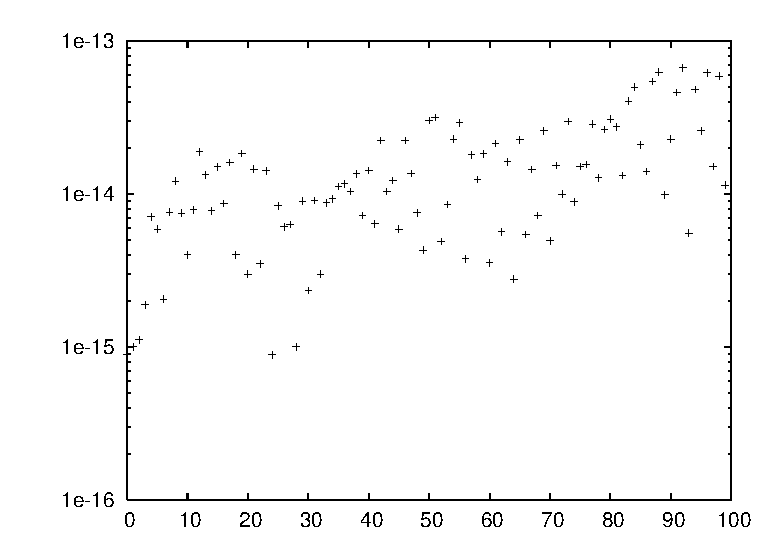
\includegraphics[width=80mm]{eps/esp-1.eps}\hfill
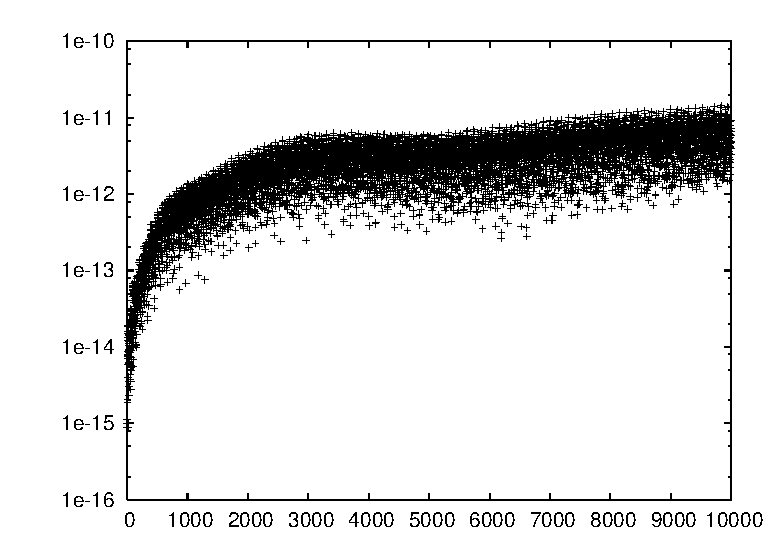
\includegraphics[width=80mm]{eps/esp-2.eps}
\caption{Error of a numerical integration of the RTBP. The horizontal
axis denotes the number of intersections with the Poincar\'e section
$z=0$. Left: the first 100 intersections. Right: 10000 intersections,
that correspond to a total integration time of 62837.969279 units. See
the text for more details.}
\label{fig:real-error}
\end{figure}

\begin{figure}
\centerline{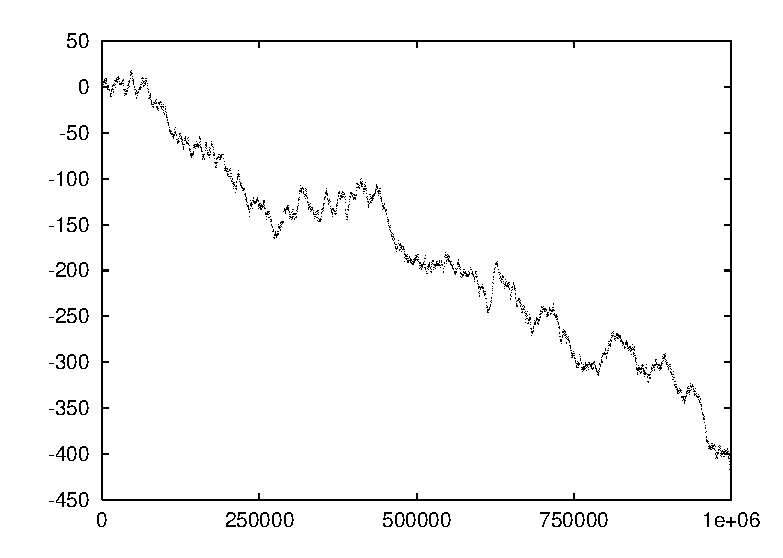
\includegraphics[width=100mm]{eps/error-h.eps}}
\caption{Long term behaviour of the energy for local thresholds
$\varepsilon_r=\varepsilon_a=10^{-16}$. Horizontal axis:
time. Vertical axis: relative variation of the value of the
Hamiltonian, in multiples of the machine precision.}
\label{fig:error-plot}
\end{figure}

As the Hamiltonian function $H$ is constant on each orbit, a second
test is simply to check for its preservation. Although the level of
preservation of $H$ does not need to be equal to the error of the
integration, checking its preservation is a common test for a
numerical integrator. Now we have selected
$\varepsilon_a=\varepsilon_r=10^{-16}$, with an integration time
of $10^6$ units. A first version of the results is shown in
Figure~\ref{fig:error-plot}, where the horizontal axis denotes the
time and the vertical axis is the difference between the actual and
the initial value of $H$, in multiples of $\eps\approx 2.22\times
10^{-16}$. Although this plot seems to indicate the presence of a bias
in the values of $H$, we want to point out that the smallness of the
drift in $H$ compared to the length of the integration time do not
allow to consider this bias meaningful from a statistical point of
view. Let us discuss this point in detail. Let $H_j$ be the value of
$H$ at the step number $j$ of the numerical integration and, instead
of consider $H_j-H_0$, let us focus on the local variation
$H_j-H_{j-1}$. In Table~\ref{tau:e-lo} we show a summary of the
results for the same trajectory as before, but for several local
thresholds for the error. To do an standard statistical analysis, let
us assume that the sequence of errors $H_j-H_{j-1}$ is given by a
sequence of independent, identically distributed random variables, and
we are interested in knowing if its mean value is zero or not.
Therefore, we will apply the following test of significance of the
mean. The null hypothesis assumes that the true mean is equal to zero.
If we define
\[
n=\sum_{|k|\le 4} \nu_k,
\]
where $k$ denotes a multiple of $\eps$ and $\nu_k$ the number of times
that this deviation has occurred, then the sample mean is
\[
m=\frac{1}{n}\sum_{|k|\le 4} k\nu_k.
\]
and the standard error of the sample mean is
\[
s=\sqrt{\frac{1}{n^2}\sum_{|k|\le 4} (k-m)^2\nu_k}.
\]
Under the previous assumptions (independence and equidistribution of
the observations), the value
\[
\tau=\frac{m}{s},
\]
must behave as a $N(0,1)$ standard normal distribution. To test the
null hypothesis (i.e., zero mean) with a confidence level of 95\%, we
have to check for the condition $|\tau|\le 1.96$. The last row of
Table~\ref{tau:e-lo} shows the value of $\tau$ for the different
integrations. It is clear that for $\varepsilon=10^{-14}$ we must
reject that the drift has zero mean, and it is also clear that this
hypothesis cannot be rejected in the other cases.

\begin{table}
\begin{center}
{\tt\small
\begin{tabular}{|r|r|r|r|r|r|}\hline
    & $\varepsilon=10^{-14}$ & $\varepsilon=10^{-15}$ &
      $\varepsilon=10^{-16}$ & $\varepsilon=10^{-17}$ &
       $\varepsilon=10^{-18}$\\ \hline
 -4 &         0 &         0 &         0 &         0 &         0\\
 -3 &        45 &         2 &         7 &         5 &         6\\
 -2 &    32,904 &    21,155 &    21,377 &    21,372 &    21,662\\
 -1 &   772,723 &   745,668 &   760,755 &   768,334 &   777,760\\
  0 & 1,970,571 & 2,084,758 & 2,134,729 & 2,157,287 & 2,174,276\\
  1 &   765,519 &   744,438 &   760,183 &   767,596 &   776,776\\
  2 &    32,444 &    21,174 &    21,576 &    21,696 &    21,949\\
  3 &        42 &         6 &         5 &         3 &         5\\
  4 &         0 &         0 &         0 &         0 &         0\\ \hline
$\tau$& -6.0613 &   -0.9160 &   -0.1383 &   -0.0735 &   -0.3141\\ \hline
\end{tabular}
}
\end{center}
\caption{Local variation of the energy for several error thresholds
$\varepsilon_a=\varepsilon_r\equiv\varepsilon$, during $10^6$ units of
time. The first column denotes multiples of the machine precision
$\eps$ and the remaining columns contain the number of integration
steps for which the local variation of energy is equal to the multiple
of eps in the first column. The last row is an statistical index to
test for zero mean, see the text for details.}
\label{tau:e-lo}
\end{table}

For the case $\varepsilon=10^{-14}$ the main source of error is
truncation that, from an statistical point of view, does not behave as
having zero mean. When the local threshold is reduced, then the main
source of error turns out to be the roundoff of the underlying
arithmetic (see Section~\ref{sec:danger}), which looks like a zero
mean random process, at least under the standard statistical tests.

A natural question is whether the Taylor method, with a sufficiently
small local threshold (like $10^{-16}$ in the previous example), can
compete with a symplectic integrator in the preservation of the
geometrical structure of the phase space of a Hamiltonian system.
From a local point of view, we want to note that the Taylor method can
deliver machine precision so it is not possible to be ``more
symplectic''. However, one has to be more careful when extending this
reasoning to long term integrations since it is possible that there
exist little biases that are only visible in very long integrations. A
deeper study is actually in progress.

\subsubsection{On the influence of the underlying arithmetic}
As an example of the effect of the arithmetic, we will show the
different behaviour of the energy. We will use the same trajectory of
the RTBP as before, and we will compute the relative variation of the
energy. The results for $\varepsilon_r=\varepsilon_a=10^{-16}$ using
the standard double precision arithmetic on different hardware are
shown in Figure~\ref{fig:error-arch}. Both graphics show that the
error behaviour seem to be dominated by the ``noise'' of the floating
point arithmetic.

\begin{figure}
\includegraphics[width=80mm]{eps/intel.eps}\hfill
\includegraphics[width=80mm]{eps/nonintel.eps}
\caption{Long term behaviour of the energy for local thresholds
  $\varepsilon_r=\varepsilon_a=10^{-16}$. Left plot: different
  optimization levels in an Intel processor (the upper curve
  corresponds to the \texttt{-O2} option). Right plot: different
  processors (the upper curve is for the AMD processor). See the text
  for more details.}
\label{fig:error-arch}
\end{figure}

\subsubsection{Extended precision calculations}\label{sec:ex-expe}
We will use the same example as in the previous section. The main
difference when generating the code for the Taylor integrator with
extended precision is that we have to tell the translator to use
extended arithmetic. For instance, to generate code using
\texttt{gmp}, we can do
\begin{verbatim}
   taylor -name rtbp -o taylor_rtbp.c -step -jet -sqrt rtbp.in
   taylor -name rtbp -o taylor.h -gmp -header
\end{verbatim}
Note that the first line is exactly the same as for the double
precision case, while the arithmetic is only specified in the
generation of the header file. The calling routine must take care of
setting the desired level of accuracy when initializing the
\texttt{gmp} package.

As a first test, we can compute the local error of a numerical
integration of the RTBP, as it has been done in
Section~\ref{sec:localerror-rtbp}. We have selected a 256 bits
mantissa (this means that the machine precision is
$\mbox{eps}=2^{-256}\approx 8.636168\times 10^{-78}$), and the value
$10^{-80}$ for both the relative and absolute error thresholds. The
method has selected a step size near $0.2$ and order 94. To obtain the
exact solution, we have used a mantissa of 512 bits and an error
threshold of $10^{-155}$. The local error of the solution after one
unit of time (this has required 4 calls to the Taylor integrator) is
shown in Table~\ref{tau:local-error-gmp}. Comparing with
Table~\ref{tau:local-error}, we see that the relative error here is a
little bit larger. We should note that the double precision arithmetic
of the Pentium processor is carried out inside registers having extra
accuracy, so it is natural to expect a slightly better behaviour for
the roundoff errors.

\begin{table}
\begin{center}
{\tt\small
\begin{tabular}{|r|r|r|r|r|r|r|}\hline
\multicolumn{1}{|c|}{$t$} & \multicolumn{1}{c|}{$e(x)$} &
\multicolumn{1}{c|}{$e(y)$} & \multicolumn{1}{c|}{$e(z)$} &
\multicolumn{1}{c|}{$e(p_x)$} & \multicolumn{1}{c|}{$e(p_y)$} &
\multicolumn{1}{c|}{$e(p_z)$} \\ \hline
1.0000000000000000 & 0.50 & -2.50 &-1.00 & -0.50 & 6.50 & -5.50\\
\hline
\end{tabular}
}
\end{center}
\caption{Local relative error (in multiples of the machine precision)
  for an orbit of the RTBP, after a unit of time, using \texttt{gmp}
  with 256 bits of mantissa. The meaning of the columns is the same as
  in Table~\ref{tau:local-error}. See the text for more comments.}
\label{tau:local-error-gmp}
\end{table}

We have also tested the variation of the value of the Hamiltonian for
a long-time integration, for different local thresholds.
Figure~\ref{fig:ham-gmp} shows the difference between the initial
value of the Hamiltonian and its value at each step of integration,
for mantissas of 128 (left) and 256 (right) bits. The differences are
shown in multiples of the machine precision of each arithmetic.  The
lower curve on these plots corresponds to the largest threshold
($\varepsilon_a=\varepsilon_r=10^{-36}$ and
$\varepsilon_a=\varepsilon_r=10^{-75}$ for the left and right plot,
respectively) where the main source of error is the truncation of the
Taylor series.  The remaining curves correspond to smaller thresholds
for which the error mainly comes from the roundoff of the \texttt{gmp}
arithmetic.  We clearly see the different behaviour of these two
sources of error, as well as the drift introduced by the roundoff of
the artihmetic.

\begin{figure}
\includegraphics[width=80mm]{eps/drift-gmp128.eps}\hfill
\includegraphics[width=80mm]{eps/drift-gmp256.eps}
\caption{Long term behaviour of the Hamiltonian for several
  integrations with \texttt{gmp} arithmetic. The horizontal axis
  displays the time and the vertical axis shows the variation of the
  Hamitonian with respect to its initial value. Left plot: results for
  \texttt{gmp} arithmetic with a 128 bits mantissa, and several local
  thresholds $\varepsilon_a=\varepsilon_r=\varepsilon$ as shown in the
  graphic. Right plot: results for \texttt{gmp} arithmetic with a 256
  bits mantissa. See the text for more details.}
\label{fig:ham-gmp}
\end{figure}

We have also tested the preservation of the Hamiltonian for a
different extended arithmetic, the \texttt{qd} library. The results
are shown in Figure~\ref{fig:ham-qd}. Again, we have used the
\texttt{dd\_real} type (two doubles) for the left plot and
\texttt{qd\_real} type (four doubles) for the right one.  For this
arithmetic, it does not make sense to use the machine precision as a
unit for the error.\footnote{A \texttt{dd\_real} number is defined as
  the sum of two doubles. Therefore, the sum $1+\varepsilon$ is always
  different from 1 as long as $\varepsilon$ can be represented in a
  double.}. Hence, we have simply multiplied the differences in the
Hamiltonian by $10^{32}$ (\texttt{dd\_real}) and $10^{64}$
(\texttt{qd\_real}). In the left plot, the bottom curve corresponds to
$\varepsilon_a=\varepsilon_r=10^{-30}$ to the largest error threshold
while the effect of the truncation dominates the error. The remaining
curves show the behaviour of the roundoff error of the arithmetic.  In
the right plot, is the upper curve that corresponds to the largest
error threshold (in this case, $\varepsilon_a=\varepsilon_r=10^{-61}$)
showing the effect of the truncation error. The remaining curves show
the drift due to the roundoff of the arithmetic.

\begin{figure}
\includegraphics[width=80mm]{eps/driftqd1.eps}\hfill
\includegraphics[width=80mm]{eps/driftqd2.eps}
\caption{Long term behaviour of the Hamiltonian for several
  integrations with \texttt{qd} arithmetic. The horizontal axis
  displays the time and the vertical axis shows the variation of the
  Hamitonian with respect to its initial value. Left plot: results for
  \texttt{dd\_real} arithmetic (nearly 32 decimal digits), and several
  local thresholds $\varepsilon_a=\varepsilon_r=\varepsilon$ as shown
  in the graphic. Right plot: results for the \texttt{qd\_real}
  arithmetic (nearly 64 decimal digits). See the text for more
  details.}
\label{fig:ham-qd}
\end{figure}


\subsection{Speed}\label{sec:sc}
There is plenty of numerical methods in the literature, and we do not
plan to survey all of them but simply to compare our implementation of
Taylor method against a few well known methods. A characteristic of
these methods is that they have a freely available implementation,
which is the one we have used. These implementations are coded in
FORTRAN77, which adds an extra difficulty on the comparisons, since
the observed differences may come from the different compilers.
Therefore, to help the readers with these comparisons, the package
includes the code for all the examples, so that they can be run on any
combination of compiler/computer for comparisons.

Our tests have been done in a GNU/Linux workstation, with an Intel
Pentium III processor running at 500 MHz. We have used the following
GNU compilers:
\begin{verbatim}
   $ gcc -v
   gcc version 2.95.4 20011002 (Debian prerelease)
   $ g77 -v
   g77 version 2.95.4 20011002 (from FSF-g77 version 0.5.25 20010319)
\end{verbatim}

The methods considered are \texttt{dop853}, an explicit Runge-Kutta
code of order 8, and \texttt{odex}, an extrapolation method of varying
order based on the Gragg-Bulirsh-Stoer algorithm. Both methods are
documented in~\cite{HairerNW00} and the code we have used is the one
contained in this book, that can be downloaded from E. Hairer's web
page, \texttt{http://www.unige.ch/math/folks/hairer/software.html}.
We note that extrapolation methods are similar to Taylor in the sense
that they can use arbitrarily high orders, so they are the natural
methods to compare with.

For the tests, we have used three vector fields: the RTBP, the Lorenz
system, a periodically forced pendulum, and the RTBP.
The equations for the Lorenz system are
\begin{eqnarray*}
\dot{x} & = & 10(y-x),\\
\dot{y} & = & x(28-z)-y,\\
\dot{z} & = & xy-\frac{8}{3}z,
\end{eqnarray*}
and the equations for the forced pendulum are
\begin{eqnarray*}
\dot{x} & = & y,\\
\dot{y} & = &-\sin(x)-0.1y+0.1\sin(t)
\end{eqnarray*}
The RTBP (see equations (\ref{eq:rtbp})) has been coded as in
Figure~\ref{fig:i-rtbp} so that, in all the cases, the vector field
has the same number of operations.

As before, we have used the same formulas to code the vector fields
for \texttt{dop853}, \texttt{odex} and \texttt{taylor}.

A first possibility to make the comparisons is to set the same
threshold for all the methods and then compare the speeds. Note that,
as the algorithms for the step size selection are completely
different, one of them could be more ``conservative'' than the others
and predict (unnecessarily) smaller step sizes so that the comparisons
would be meaningless. For this reason we have proceeded in the
following way: given an initial condition, we can compute the
corresponding orbit during, say, 16 units of time and to compare the
final point with the true value to obtain the real absolute
error.\footnote{The true value has been obtained from an integration
  with the Taylor method using the \texttt{gmp} arithmetic with
  mantissas of 128 and 256 bits.} In Table~\ref{tau:speed} we show the
computer time and final error for the three methods, using different
thresholds for the step size control. To have a measurable running
time, the program repeats the same calculation 1000 times.

Therefore, we ignore the column labelled $\varepsilon$ (the error
threshold used for the step size control), and we only compare the
computing time to achieve a prescribed accuracy (this is equivalent to
compare the accuracy obtained for a fixed computing time). The results
clearly show the effectiveness of the Taylor method for these
examples.

\begin{table}
\begin{center}
{\tt
\begin{tabular}{|r|r|r||r|r|r||r|r|r|}\hline
\multicolumn{9}{|c|}{\textrm{Lorenz}} \\ \hline
\multicolumn{3}{|c||}{\texttt{dop583}} &
\multicolumn{3}{c||}{\texttt{odex}} &
\multicolumn{3}{c|}{\texttt{taylor}} \\ \hline
\multicolumn{1}{|c|}{$\varepsilon$} &
\multicolumn{1}{|c|}{\textrm{time}} &
\multicolumn{1}{|c||}{\textrm{error}} &
\multicolumn{1}{|c|}{$\varepsilon$} &
\multicolumn{1}{|c|}{\textrm{time}} &
\multicolumn{1}{|c||}{\textrm{error}} &
\multicolumn{1}{|c|}{$\varepsilon$} &
\multicolumn{1}{|c|}{\textrm{time}} &
\multicolumn{1}{|c|}{\textrm{error}}\\ \hline
1.e-10 &  7.01 & 5.9e-03 & 1.e-10 &  8.73 & 6.2e-02 & 1.e-10 & 7.61 & 3.1e-06\\
1.e-11 &  8.91 & 5.0e-04 & 1.e-11 & 10.11 & 3.3e-03 & 1.e-11 & 7.99 & 4.4e-07\\
1.e-12 & 11.65 & 4.3e-05 & 1.e-12 & 11.54 & 2.0e-04 & 1.e-12 & 8.40 & 4.8e-08\\
1.e-13 & 15.31 & 3.7e-06 & 1.e-13 & 12.74 & 5.8e-06 & 1.e-13 & 8.80 & 3.3e-08\\
1.e-14 & 20.19 & 1.2e-06 & 1.e-14 & 15.04 & 6.4e-06 & 1.e-14 & 9.22 & 3.4e-08\\
1.e-15 & 26.76 & 8.9e-07 & 1.e-15 & 17.81 & 3.7e-06 & 1.e-15 & 9.75 & 9.2e-09\\
1.e-16 & 35.51 & 9.5e-07 & 1.e-16 & 50.47 & 1.9e-06 & 1.e-16 &10.75 & 7.5e-09\\
\hline\hline
\multicolumn{9}{|c|}{\textrm{Perturbed pendulum}} \\ \hline
\multicolumn{3}{|c||}{\texttt{dop583}} &
\multicolumn{3}{c||}{\texttt{odex}} &
\multicolumn{3}{c|}{\texttt{taylor}} \\ \hline
\multicolumn{1}{|c|}{$\varepsilon$} &
\multicolumn{1}{|c|}{\textrm{time}} &
\multicolumn{1}{|c||}{\textrm{error}} &
\multicolumn{1}{|c|}{$\varepsilon$} &
\multicolumn{1}{|c|}{\textrm{time}} &
\multicolumn{1}{|c||}{\textrm{error}} &
\multicolumn{1}{|c|}{$\varepsilon$} &
\multicolumn{1}{|c|}{\textrm{time}} &
\multicolumn{1}{|c|}{\textrm{error}}\\ \hline
1.e-10 & 0.62 & 3.4e-11 & 1.e-10 & 1.49 & 6.9e-10 & 1.e-10 & 0.38 & 2.8e-13\\
1.e-11 & 0.78 & 3.6e-12 & 1.e-11 & 1.70 & 4.9e-11 & 1.e-11 & 0.42 & 2.1e-14\\
1.e-12 & 1.03 & 3.1e-13 & 1.e-12 & 1.93 & 1.7e-12 & 1.e-12 & 0.44 & 7.6e-15\\
1.e-13 & 1.38 & 2.7e-14 & 1.e-13 & 2.17 & 9.1e-14 & 1.e-13 & 0.47 & 1.2e-15\\
1.e-14 & 1.83 & 2.3e-15 & 1.e-14 & 2.36 & 4.4e-15 & 1.e-14 & 0.48 & 8.7e-16\\
1.e-15 & 2.45 & 2.1e-15 & 1.e-15 & 2.68 & 3.1e-15 & 1.e-15 & 0.52 & 5.8e-16\\
1.e-16 & 3.24 & 3.2e-15 & 1.e-16 & 3.09 & 1.1e-14 & 1.e-16 & 0.59 & 3.8e-16\\
\hline\hline
\multicolumn{9}{|c|}{\textrm{RTBP}} \\ \hline
\multicolumn{3}{|c||}{\texttt{dop583}} &
\multicolumn{3}{c||}{\texttt{odex}} &
\multicolumn{3}{c|}{\texttt{taylor}} \\ \hline
\multicolumn{1}{|c|}{$\varepsilon$} &
\multicolumn{1}{|c|}{\textrm{time}} &
\multicolumn{1}{|c||}{\textrm{error}} &
\multicolumn{1}{|c|}{$\varepsilon$} &
\multicolumn{1}{|c|}{\textrm{time}} &
\multicolumn{1}{|c||}{\textrm{error}} &
\multicolumn{1}{|c|}{$\varepsilon$} &
\multicolumn{1}{|c|}{\textrm{time}} &
\multicolumn{1}{|c|}{\textrm{error}}\\ \hline
1.e-10 & 1.43 & 1.1e-09 & 1.e-10 & 1.74 & 1.8e-09 & 1.e-10 & 1.68 & 6.2e-12\\
1.e-11 & 1.84 & 9.4e-11 & 1.e-11 & 2.02 & 9.2e-11 & 1.e-11 & 1.86 & 4.6e-13\\
1.e-12 & 2.44 & 8.6e-12 & 1.e-12 & 2.43 & 2.4e-11 & 1.e-12 & 2.08 & 4.4e-14\\
1.e-13 & 3.24 & 8.0e-13 & 1.e-13 & 2.74 & 3.7e-13 & 1.e-13 & 2.27 & 7.2e-15\\
1.e-14 & 4.32 & 7.5e-14 & 1.e-14 & 3.14 & 1.5e-13 & 1.e-14 & 2.50 & 4.2e-15\\
1.e-15 & 5.73 & 9.9e-15 & 1.e-15 & 3.71 & 2.4e-13 & 1.e-15 & 2.82 & 1.7e-15\\
1.e-16 & 7.63 & 2.0e-15 & 1.e-16 & 4.85 & 1.3e-13 & 1.e-16 & 3.26 & 5.8e-15\\
\hline
\end{tabular}
}
\end{center}
\caption{Speed comparison between \texttt{dopri853}, \texttt{odex} and
\texttt{taylor}. $\varepsilon$ is the selected threshold for the error
(both relative and absolute thresholds have been set to the same
value), computer time is given in seconds, and the error is the
absolute error at the end point of the integration. To have a
measurable computer time, we have repeated the same integration 1000
times. See the text for more details.}
\label{tau:speed}
\end{table}

\subsubsection{A simple comparison with ADOL-C}
ADOL-C is a public domain package for automatic differentiation. The
main differences between the automatic differentiation of our package
and ADOL-C are:
\begin{itemize}
\renewcommand{\itemsep}{0pt}
\item[a)] ADOL-C is a general purpose package, while \texttt{taylor}
is specifically designed for the numerical integration of ODEs.

\item[b)] The input of ADOL-C is a C/C++ function (with some
restrictions in the grammar used), while \texttt{taylor} has its own
input grammar, which is a little bit more restrictive.

\item[c)] ADOL-C does not include code for the step size control. This
means that ADOL-C can only be used to generate the Taylor coefficients
and the user must supply code for the order and step size control.

For this reason, we will only test the speed of the generation of the
Taylor coefficients.
\end{itemize}

As before, the tests have been done on an Intel Pentium III running at
500 MHz, using ADOL-C version 1.8.7. The examples considered are the
Lorenz system, RTBP, the Lorenz system and a periodically forced
pendulum. To measure the time, we have computed the jet of derivatives
100,000 times. The results are contained in
Table~\ref{tau:adolc-taylor}, and clearly show the efficiency of
\texttt{taylor}.

\begin{table}
\begin{center}
{\tt
\begin{tabular}{|c|r|r|r|r|}\hline
   &
  \multicolumn{1}{c|}{\textrm{degree}} &
  \multicolumn{1}{c|}{\textrm{Lorenz}} &
  \multicolumn{1}{c|}{\textrm{Pendulum}} &
   \multicolumn{1}{c|}{\textrm{RTBP}} \\ \hline\hline
\textrm{ADOL-C} & 40 & 92.82 & 140.57 & 403.22\\ \hline
\textrm{Taylor} & 40 &  3.59 &   3.43 &  14.75\\ \hline\hline
\textrm{ADOL-C} & 20 & 24.44 &  34.82 &  87.99\\ \hline
\textrm{Taylor} & 20 &  1.13 &   1.07 &   4.65\\ \hline\hline
\textrm{ADOL-C} & 10 &  9.13 &  11.58 &  26.20\\ \hline
\textrm{Taylor} & 10 &  0.41 &   0.39 &   1.62\\ \hline
\end{tabular}
}
\end{center}
\caption{Time (in seconds) to compute 100,000 times the jet of
  derivatives for the Lorenz system, a periodically
  forced pendulum and the RTBP.}
\label{tau:adolc-taylor}
\end{table}


\section{Conclusions}
In this paper we have discussed a new publicly available
implementation of the classical Taylor method for the numerical
solution of ODEs. This program reads the differential equations from a
file and outputs a complete Taylor integrator (including adaptive
selection of degree and step size) for the given system.

The package has been tested against freely available implementations
of two well-known numerical integrators. We do not claim that the
results from these tests can be extrapolated to any example, but
simply that \texttt{taylor} can be very competitive in many
situations. We believe that the fact that the the methods used for the
comparisons are coded in FORTRAN 77 while the output of
\texttt{taylor} is ANSI C has a small impact in the results. However,
the package includes the source code used for tests, so that the user
can try them with different compilers/computers. In fact, the best way
to know whether \texttt{taylor} is suitable for a concrete
application, with a given compiler and computer, is simply to try it.

Finally, let us remark that one of the strong points of the package
is the support for extended precision arithmetic.


\section*{Acknowledgements}
The authors want to thank R. Broucke, R. de la Llave and C. Sim\'o for
their comments. This work has been supported by the Comisi\'on
Conjunta Hispano Norteamericana de Cooperaci\'on Cient\'{\i}fica y
Tecnol\'ogica. A.J. has also been supported by the MCyT/FEDER grant
BFM2003-07521-C02-01, the Catalan CIRIT grant 2001SGR--70 and DURSI.

\addcontentsline{toc}{section}{References}
\bibliographystyle{alpha}
\bibliography{ds,na}

\end{document}
